% !TeX root = ../main.tex

% Edit this title for each week's entry.
\section{Week 3: Assumptions of Linear Regression Models}

\noindent\fbox{\begin{minipage}{\dimexpr\linewidth-2\fboxsep-2\fboxrule}
\textbf{Learning Objectives}
\begin{itemize}
    \item[\textit{Basic}] State the 4 linear regression assumptions and
    what each means \S\ref{def:assumptions}; use residual plots and QQ
    plots to check them \S\ref{sec:residplots}.
    \item[\textit{Adv.}] Explain why residuals have non-constant variance
    and when to standardize; check the two extra conditions needed before
    residual plots can be trusted in MLR \S\ref{sec:mlrconditions}.
\end{itemize}
\end{minipage}}

\subsection{Review: MLR, Indicators and Interactions}

\begin{remark}[MLR in Matrix Form]
    $Y_i=\beta_0+\beta_1x_{i1}+\cdots+\beta_px_{ip}+\epsilon_i=\mathbf{x}_i'\boldsymbol\beta+\epsilon_i$,
    $\epsilon_i\overset{iid}\sim N(0,\sigma^2)$, i.e.\
    $\mathbf{Y}=\mathbf{X}\boldsymbol\beta+\boldsymbol\epsilon$ with
    $\boldsymbol\epsilon\sim N(\mathbf{0}_n,\sigma^2\mathbf{I}_n)$.
    \aside{$\mathbf{Y}$ = column vector of responses; $\mathbf{X}$ = design
    matrix; $N(\mathbf{0}_n,\sigma^2\mathbf{I}_n)$ = multivariate normal.}
\end{remark}

\begin{example}[Design Matrix with Interaction --- \texttt{mtcars}]
    \texttt{lm(mpg \textasciitilde\ wt * factor(cyl))} fits
    \[mpg=\beta_0+\beta_1wt+\underbrace{\beta_2\mathbb{I}(cyl=6)+\beta_3\mathbb{I}(cyl=8)}_{\text{main effect for cyl}}
    +\underbrace{\beta_4wt\cdot\mathbb{I}(cyl=6)+\beta_5wt\cdot\mathbb{I}(cyl=8)}_{\text{interaction wt}\times\text{cyl}}+\epsilon\]
    \texttt{model.matrix()} has columns $1,\ X_1=wt,\ X_2=\mathbb{I}(cyl=6),\ X_3=\mathbb{I}(cyl=8),\ X_4=X_1X_2,\ X_5=X_1X_3$.
    \aside{Main effect $\Rightarrow$ different \emph{intercepts} per group;
    interaction $\Rightarrow$ different \emph{slopes} per group.}
    Fitted: $\hat\beta_0=39.571$, $\hat\beta_1=-5.647$, $\hat\beta_2=-11.162$,
    $\hat\beta_3=-15.703$, $\hat\beta_4=2.867$, $\hat\beta_5=3.455$
    ($R^2=0.8616$).
\end{example}

\subsection{Linear Regression Assumptions}

\begin{remark}[Why We Need Assumptions]
    $Y_1,\dots,Y_n$ are random; treat $\mathbf{X}_1,\dots,\mathbf{X}_n$ as
    fixed. So $\hat{\boldsymbol\beta}=(\mathbf{X}'\mathbf{X})^{-1}\mathbf{X}'\mathbf{Y}$
    is random, with a \textbf{sampling distribution} (like $\hat\mu$ in 2nd
    year). We need assumptions to determine that sampling distribution, to
    have a valid model fit, and to make statistical inferences.
\end{remark}

\begin{example}[Anscombe's Quartet]
    Anscombe (1973) built 4 datasets (in R: \texttt{anscombe}) with nearly
    identical summary statistics:
    \[\bar x=9,\quad \bar y\approx7.5,\quad \Var(x)=11,\quad \Var(y)\approx4.13,\quad \text{corr}(x,y)\approx0.82,\quad \hat y=3+0.5x\]
    for \emph{all four}, yet they look completely different when plotted.
    \aside{Always graph your data! See Sheather \S3.1 (pg 45).}
    \begin{center}
        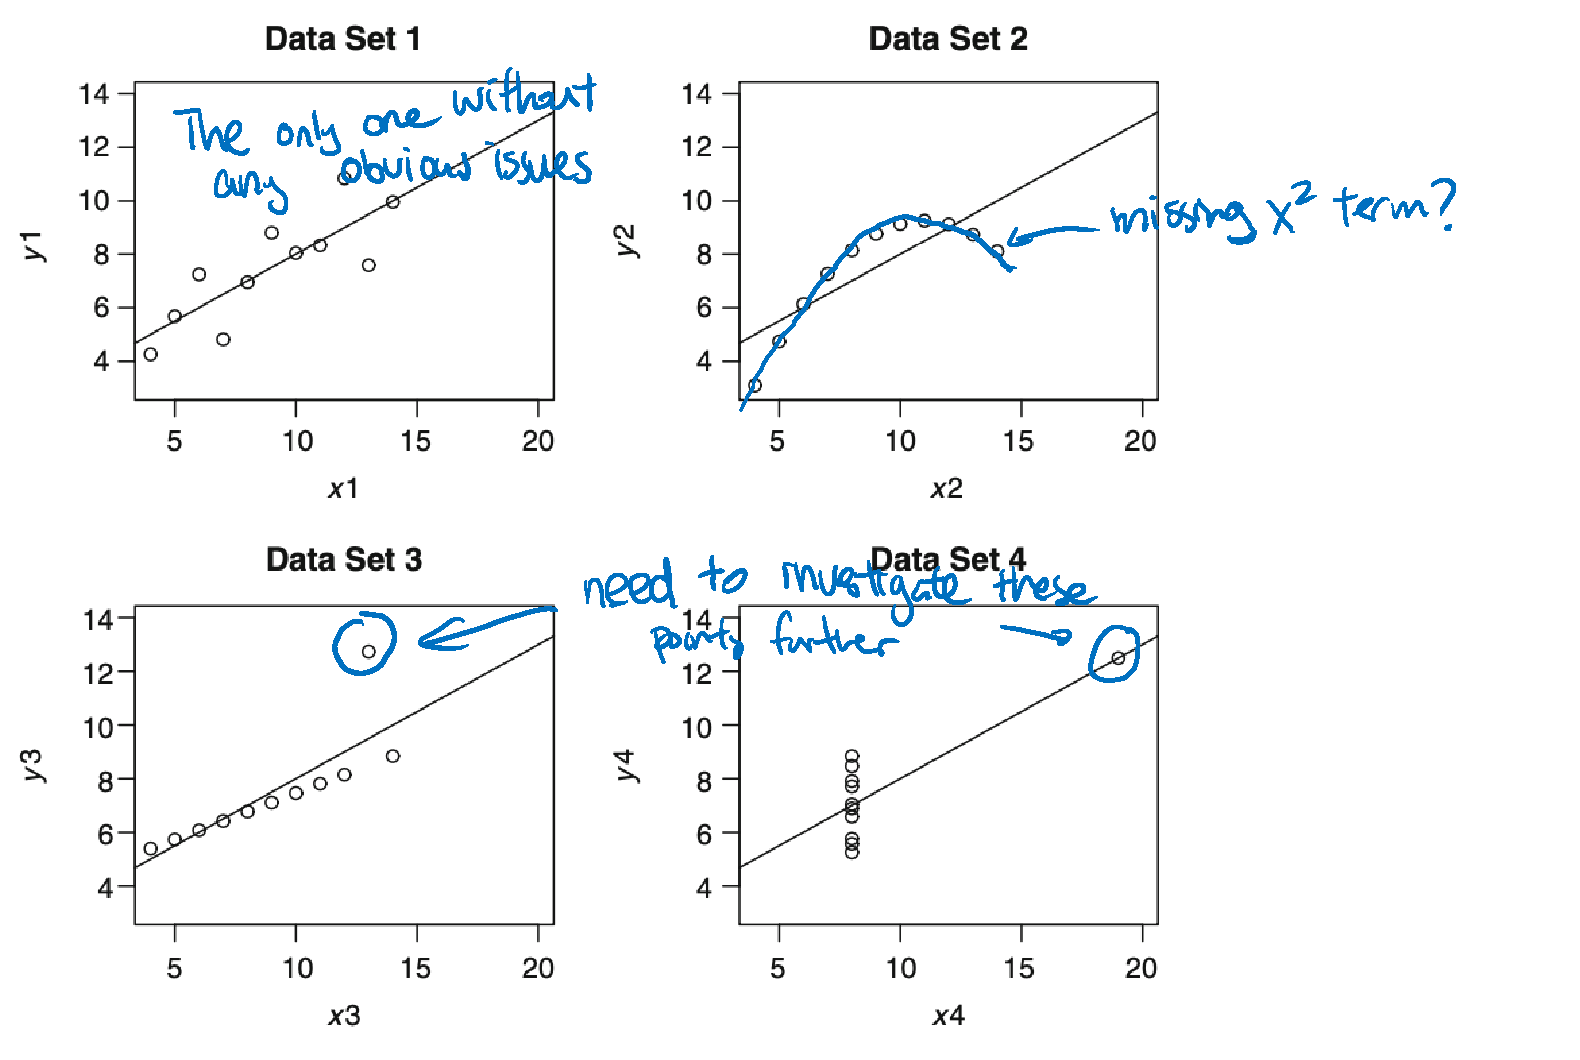
\includegraphics[width=0.72\linewidth]{figures/anscombe_scatter.png}
    \end{center}
    \aside{Set 1: the only one without obvious issues. Set 2: missing an
    $x^2$ term? Sets 3 \& 4: need to investigate the circled points further.}
\end{example}

\begin{remark}
    ``All models are wrong, but some are useful'' --- George Box (1976).
\end{remark}

\begin{definition}[The 4 Assumptions]\label{def:assumptions}
    Assumptions are about the \textbf{population}, not the sample, and we
    implicitly make them \textbf{every} time we fit a model.
    \begin{enumerate}
        \item \textbf{Linearity} (a.k.a.\ \textbf{mean zero errors}):
        $E(\boldsymbol\epsilon\mid\mathbf{X})=\mathbf{0}$, i.e.\
        $E(\mathbf{Y}\mid\mathbf{X})=\mathbf{X}\boldsymbol\beta$
        \item \textbf{Uncorrelated errors} (a.k.a.\ independence, no
        autocorrelation, no serial correlation):
        $\Cov(\epsilon_i,\epsilon_j)=\Cov(y_i,y_j)=0$ for $i\neq j$
        \item \textbf{Constant error variance} (\textbf{homoskedasticity}):
        $\Var(\boldsymbol\epsilon\mid\mathbf{X})=\Var(\mathbf{Y}\mid\mathbf{X})=\sigma^2\mathbf{I}$,
        i.e.\ $\Var(\epsilon_i\mid X)=\sigma^2$
        \item \textbf{Normal errors}:
        $\boldsymbol\epsilon\mid\mathbf{X}\sim N_n(\mathbf{0}_n,\sigma^2\mathbf{I}_n)$,
        i.e.\ $\epsilon_i\overset{iid}\sim N(0,\sigma^2)$
    \end{enumerate}
    \aside{The single statement $\boldsymbol\epsilon\mid\mathbf{X}\sim N_n(\mathbf{0}_n,\sigma^2\mathbf{I}_n)$
    implies all 4 assumptions. Normality is technically not needed for OLS,
    but is needed for inference on $\boldsymbol\beta$.}
\end{definition}

\begin{center}
    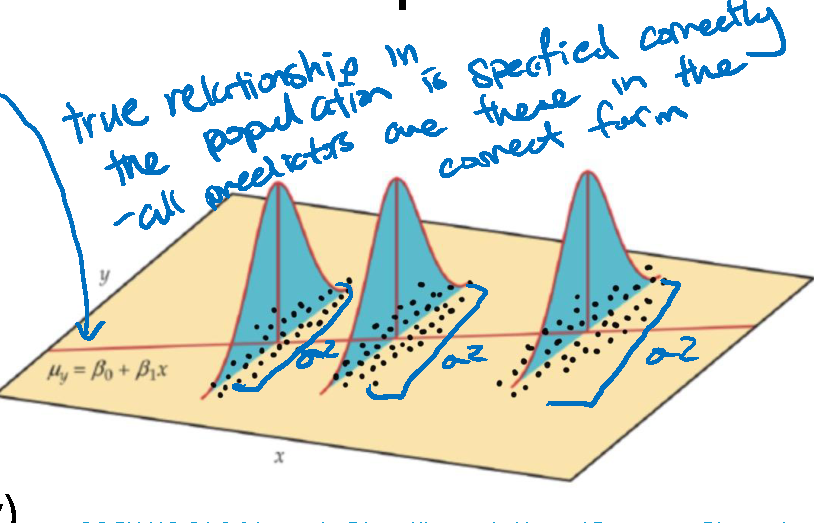
\includegraphics[width=0.5\linewidth]{figures/assumptions_picture.png}
    \\[2pt] \textit{\small Each conditional distribution of $Y$ is normal, centred on the line, with the same spread $\sigma^2$.}
\end{center}

\heading{What Each Assumption Means}
\begin{itemize}
    \item \rb{Linearity / mean zero errors}: the true relationship is
    linear in the \emph{coefficients}, and is exactly
    $\mathbf{Y}=\mathbf{X}\boldsymbol\beta+\boldsymbol\epsilon$ with
    \begin{itemize}
        \item no predictors omitted from $\mathbf{X}$ that should be present,
        \item no predictors included in $\mathbf{X}$ that should not be present,
        \item no predictors in $\mathbf{X}$ in the wrong functional form
        \aside{($x$ is transformed if necessary)}.
    \end{itemize}
    Violations: omitting a predictor known to influence the response;
    fitting a linear model when the truth is $y_i=\log(\beta_0+\beta_1x_i+\epsilon_i)$;
    including $x$ when it should be $x+x^2$.
    \aside{U-shaped data: $Y=\beta_0+\beta_1x$ violates linearity, but
    $Y=\beta_0+\beta_1x+\beta_2x^2$ is fine --- still linear in $\boldsymbol\beta$.}
    \item \rb{Uncorrelated errors}: no data point in the population is
    related to any other (knowing one tells you nothing about another).
    Depends on \emph{how samples are taken}. Violations: stock prices,
    weather data, repeated measurements on the same person, family/social
    groups.
    \item \rb{Constant variance}: each conditional distribution has the
    same \emph{spread}; the only difference between conditional
    distributions of $Y_i$ is that the mean shifts.
    \item \rb{Normality}: each conditional distribution has the same
    (normal) \emph{shape}. Harder to verify in small samples
    \aside{--- but also more important in small samples}. \textbf{Not}
    needed to estimate coefficients by least squares (the normal
    distribution is never used in that derivation).
\end{itemize}

\heading{Importance of Assumptions}
\begin{itemize}
    \item Linearity $\Rightarrow$ coefficients are estimated \textbf{unbiasedly}
    \item Uncorrelated errors $\Rightarrow$ correct \textbf{precision} of estimates
    \item Constant variance $\Rightarrow$ reasonable estimates of variability for all conditional means
    \item Normality $\Rightarrow$ can use properties of normal RVs for \textbf{inference} (e.g.\ CIs)
    \item Nothing stops us from fitting an invalid model with violated assumptions!
\end{itemize}

\subsection{Verifying Assumptions with Residual Plots}\label{sec:residplots}

\begin{definition}[Residuals]
    $\hat{\boldsymbol\epsilon}=\mathbf{Y}-\hat{\mathbf{Y}}=(\mathbf{I}_n-\mathbf{H})\mathbf{Y}$
    are our (sample) estimates of the errors, with
    \[E[\hat\epsilon_i\mid X]=0, \qquad \Var[\hat\epsilon_i\mid X]=\sigma^2(1-h_{ii}),\]
    where $h_{ii}$ is the $i$-th diagonal entry of
    $\mathbf{H}=\mathbf{X}(\mathbf{X}'\mathbf{X})^{-1}\mathbf{X}'$.
    \aside{The errors all have the same variance, but the residuals'
    variances depend on $X$.} Estimate $\sigma^2$ by
    \[\hat\sigma^2 = \frac{1}{n-(p+1)}\sum_{i=1}^n\big(Y_i-\hat Y_i\big)^2 = \frac{1}{n-(p+1)}\sum_{i=1}^n\hat\epsilon_i^2\]
    \aside{df $=n-p-1$: $n$ observations minus $p+1$ $\beta$'s. The sum is
    the same as in SLR.}
\end{definition}

\begin{definition}[Standardized Residuals]
    Since residuals don't all have the same variance, standardize:
    \[r_i = \frac{\hat\epsilon_i}{\hat\sigma\sqrt{1-h_{ii}}}\]
\end{definition}

\begin{proposition}[$0\le h_{ii}\le1$]
    $\mathbf{H}$ is a projection matrix, so $\mathbf{H}=\mathbf{H}^2$, giving
    \[h_{ii}=h_{ii}^2+\sum_{j\neq i}h_{ij}^2 \ \Rightarrow\ h_{ii}\ge h_{ii}^2 \ \Rightarrow\ 0\le h_{ii}\le1.\]
    If $h_{ii}\approx1$ (extremely high leverage), $\hat\epsilon_i$ has
    variance $\approx0$, so it is forced close to 0.
    \aside{Most $h_{ii}$ will be small (close to 0).}
    Standardized residual plots are more informative when high-leverage
    points exist. \aside{Often, regular residual plots are used.}
\end{proposition}

\begin{remark}[Why Residuals Reveal Violations]
    With population errors $\epsilon_i=y_i-E(y_i\mid x_i)$ and residuals
    $\hat\epsilon_i=y_i-\hat E(y_i\mid x_i)$: residuals capture the noise
    left over after estimating the trend. If $\hat{\boldsymbol\beta}\approx\boldsymbol\beta$,
    \[\underbrace{\hat{\boldsymbol\epsilon}}_{\text{observed}}=\mathbf{Y}-\hat{\mathbf{Y}}=\mathbf{X}(\boldsymbol\beta-\hat{\boldsymbol\beta})+\boldsymbol\epsilon\approx\underbrace{\boldsymbol\epsilon}_{\text{unobserved}}\]
    So violations show up in the residuals. E.g.\ if the truth is
    $y_i=\beta_0+\beta_1x_{i1}+\beta_2x_{i1}^2+\epsilon_i$ but we fit
    $\hat y_i=\hat\beta_0+\hat\beta_1x_{i1}$:
    \[\hat\epsilon_i=(\beta_0-\hat\beta_0)+(\beta_1-\hat\beta_1)x_{i1}+\beta_2x_{i1}^2+\epsilon_i\approx\beta_2x_{i1}^2+\epsilon_i\]
    \aside{Residuals show what was missed in your specified model.}
\end{remark}

\heading{What Good Residuals Look Like}
\begin{itemize}
    \item Uncorrelated with the fitted values and predictors \aside{(no patterns)}
    \item Residuals vs.\ fitted values or any predictor have \textbf{constant} mean 0
    \item \textbf{No systematic patterns} \aside{--- should look like a random cloud}
    \item Roughly normally distributed \aside{A funnel (spread growing with $x$ or $\hat y$) violates constant variance.}
\end{itemize}

\begin{remark}[No Perfect Diagnostic]
    Diagnostic plots may not capture violations, and may be misleading
    (especially for small $n$; more trustworthy for large $n$). A
    violation of one assumption may affect the diagnostic plot for
    \emph{another} assumption.
\end{remark}

\begin{center}
    \begin{tabular}{ll}
        \toprule
        Plot & Checks \\
        \midrule
        Residuals vs.\ fitted values (scatter) & linearity, uncorrelated errors, constant variance \\
        Residuals vs.\ each predictor (scatter) & linearity, uncorrelated errors, constant variance \\
        Histogram of (standardized) residuals & normality, mean zero \\
        Normal QQ plot of residuals & normality \\
        \bottomrule
    \end{tabular}
    \\[2pt] \textit{\small Any of these can use standardized residuals instead.}
\end{center}

\begin{example}[You Try]
    Scatterplots with line of best fit (left) and residuals vs.\ fitted
    (right) for two datasets. What patterns do we see?
    \begin{center}
        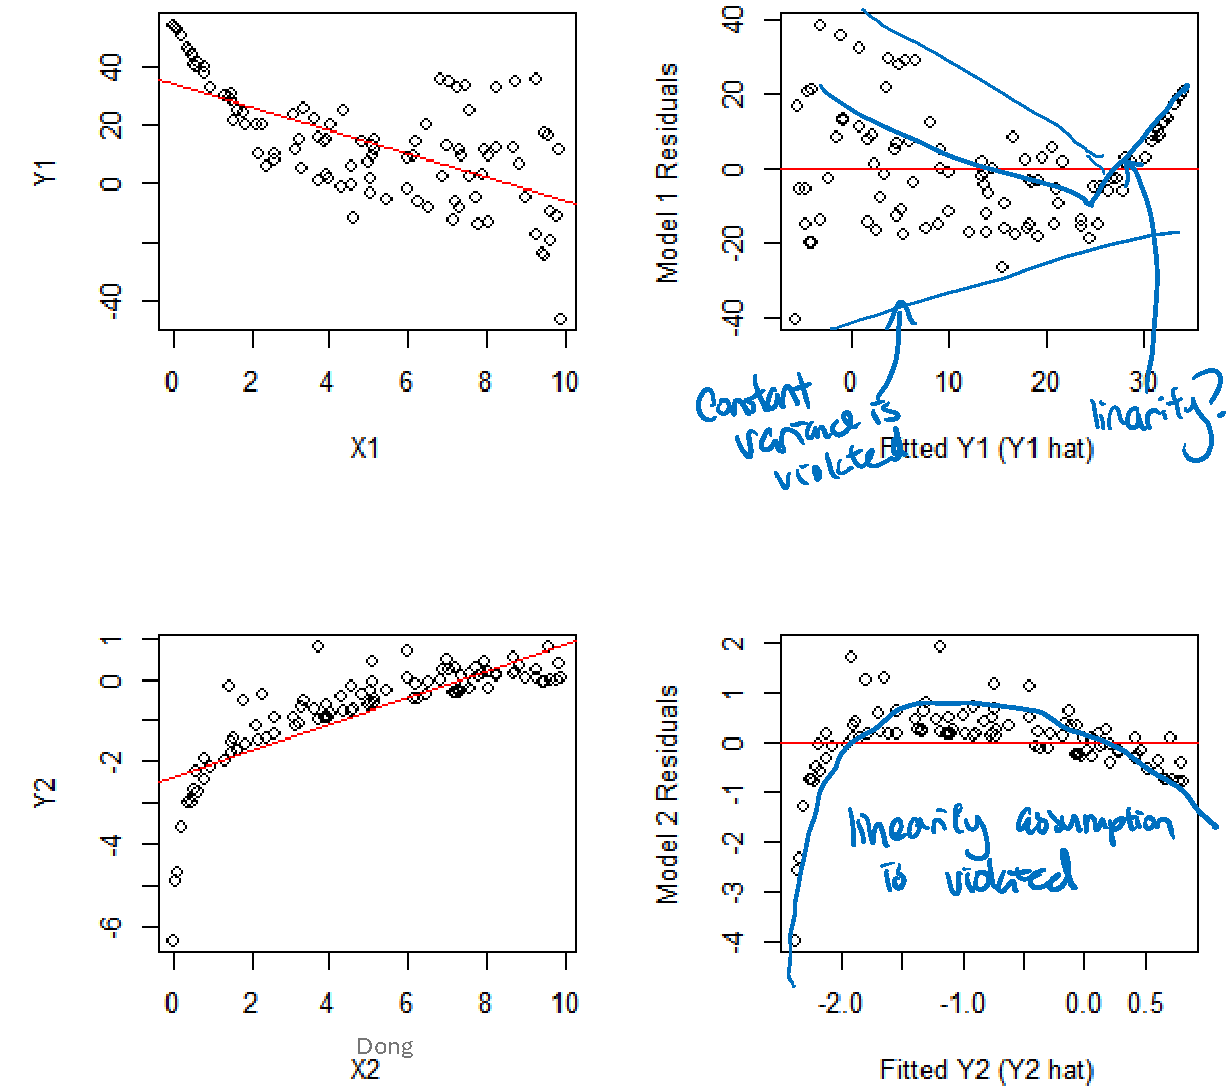
\includegraphics[width=0.62\linewidth]{figures/you_try_residuals.png}
    \end{center}
    \db{$(X_1,Y_1)$: the residuals fan out, so \dbb{constant variance is violated};
    the curve on the right also suggests a linearity problem.
    $(X_2,Y_2)$: the residuals follow an arch, so \dbb{linearity is violated}.}
\end{example}

\begin{definition}[Normal QQ Plot]
    To check normality with a QQ plot of the $r_i$:
    \begin{enumerate}
        \item Sort the data from smallest to largest; record the percentile each value occupies.
        \item Find the standard normal quantile ($z$-score) at the same percentiles.
        \item Plot each data point $x_i$ against its $z_i$.
    \end{enumerate}
    If the distribution is close to normal, the points form a
    \textbf{straight line}. In R: \texttt{qqnorm(model\$residuals)} and
    \texttt{qqline(model\$residuals)}.
\end{definition}

\begin{remark}[Reading QQ Plots]
    Typical deviations from a straight line:
    \begin{itemize}
        \item \textbf{Outliers}: odd values far from the rest
        \item \textbf{Curvature at both ends}: long (heavy) or short (light) tails
        \item \textbf{Convex/concave curvature}: asymmetry/skewness
        \item \textbf{Horizontal segments, plateaus, gaps} (e.g.\ bimodal)
    \end{itemize}
\end{remark}

\begin{center}
    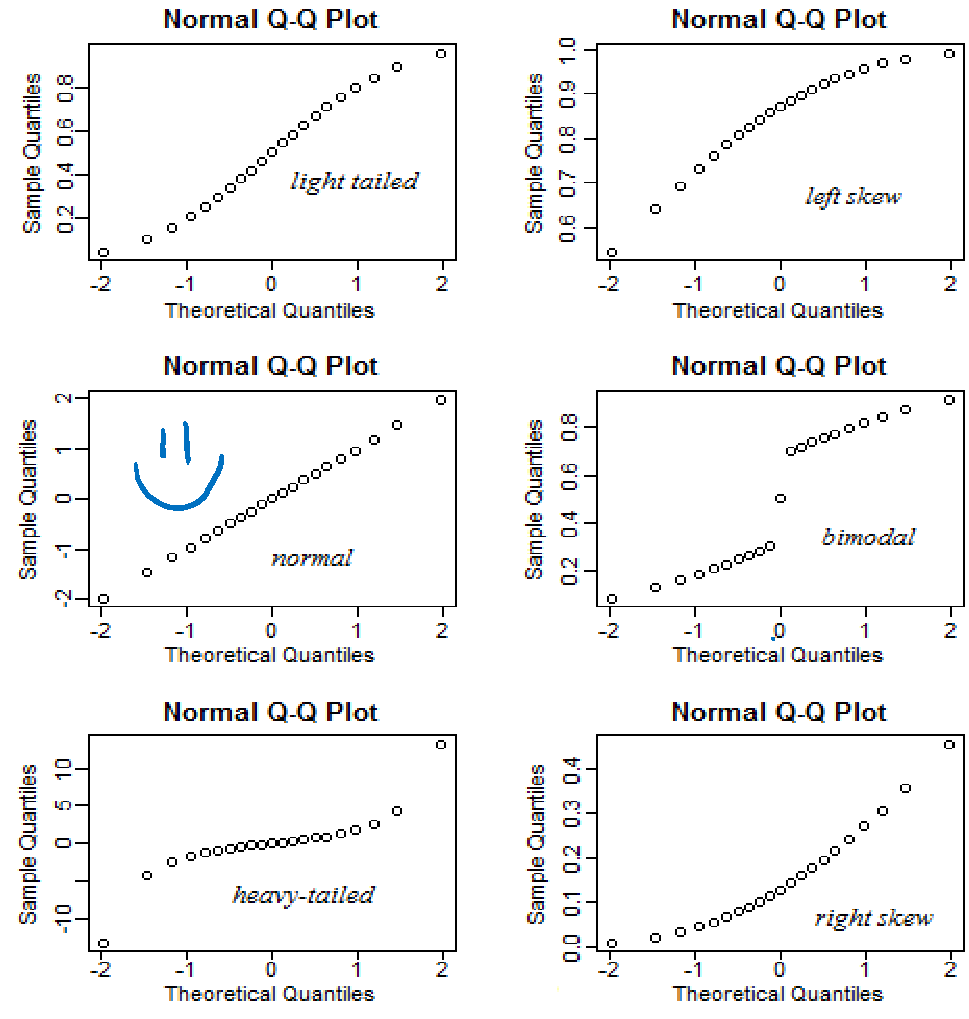
\includegraphics[width=0.55\linewidth]{figures/qq_shapes.png}
\end{center}

\begin{example}[Back to Anscombe's Quartet]
    For each dataset: scatter with fit, residuals vs.\ fitted, residuals
    vs.\ predictor, normal QQ plot.
\begin{verbatim}
model1 <- lm(y1 ~ x1, data = anscombe)
y_hat <- fitted(model1); e_hat <- resid(model1)
par(mfrow = c(2, 2))   # 2x2 grid of plots
plot(anscombe$x1, anscombe$y1); abline(model1, col = "red")
plot(y_hat, e_hat)            # residuals vs fitted
plot(anscombe$x1, e_hat)      # residuals vs predictor
qqnorm(e_hat); qqline(e_hat)
\end{verbatim}
    \begin{center}
        \begin{minipage}{0.48\linewidth}\centering
            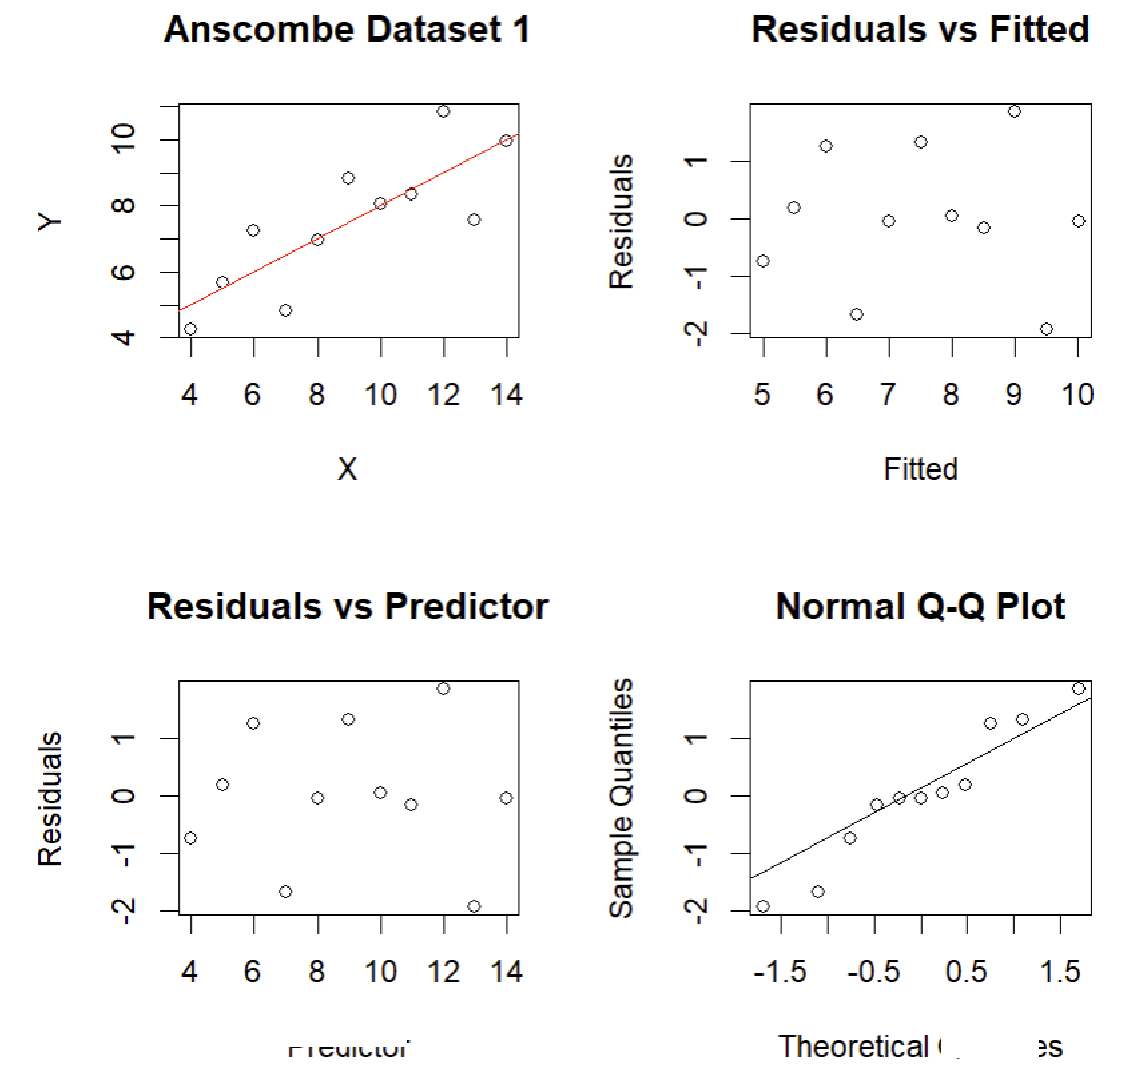
\includegraphics[width=\linewidth]{figures/anscombe1_diag.png}
            \\ \textit{\small Set 1: random cloud, QQ roughly straight --- no issues}
        \end{minipage}
        \hfill
        \begin{minipage}{0.48\linewidth}\centering
            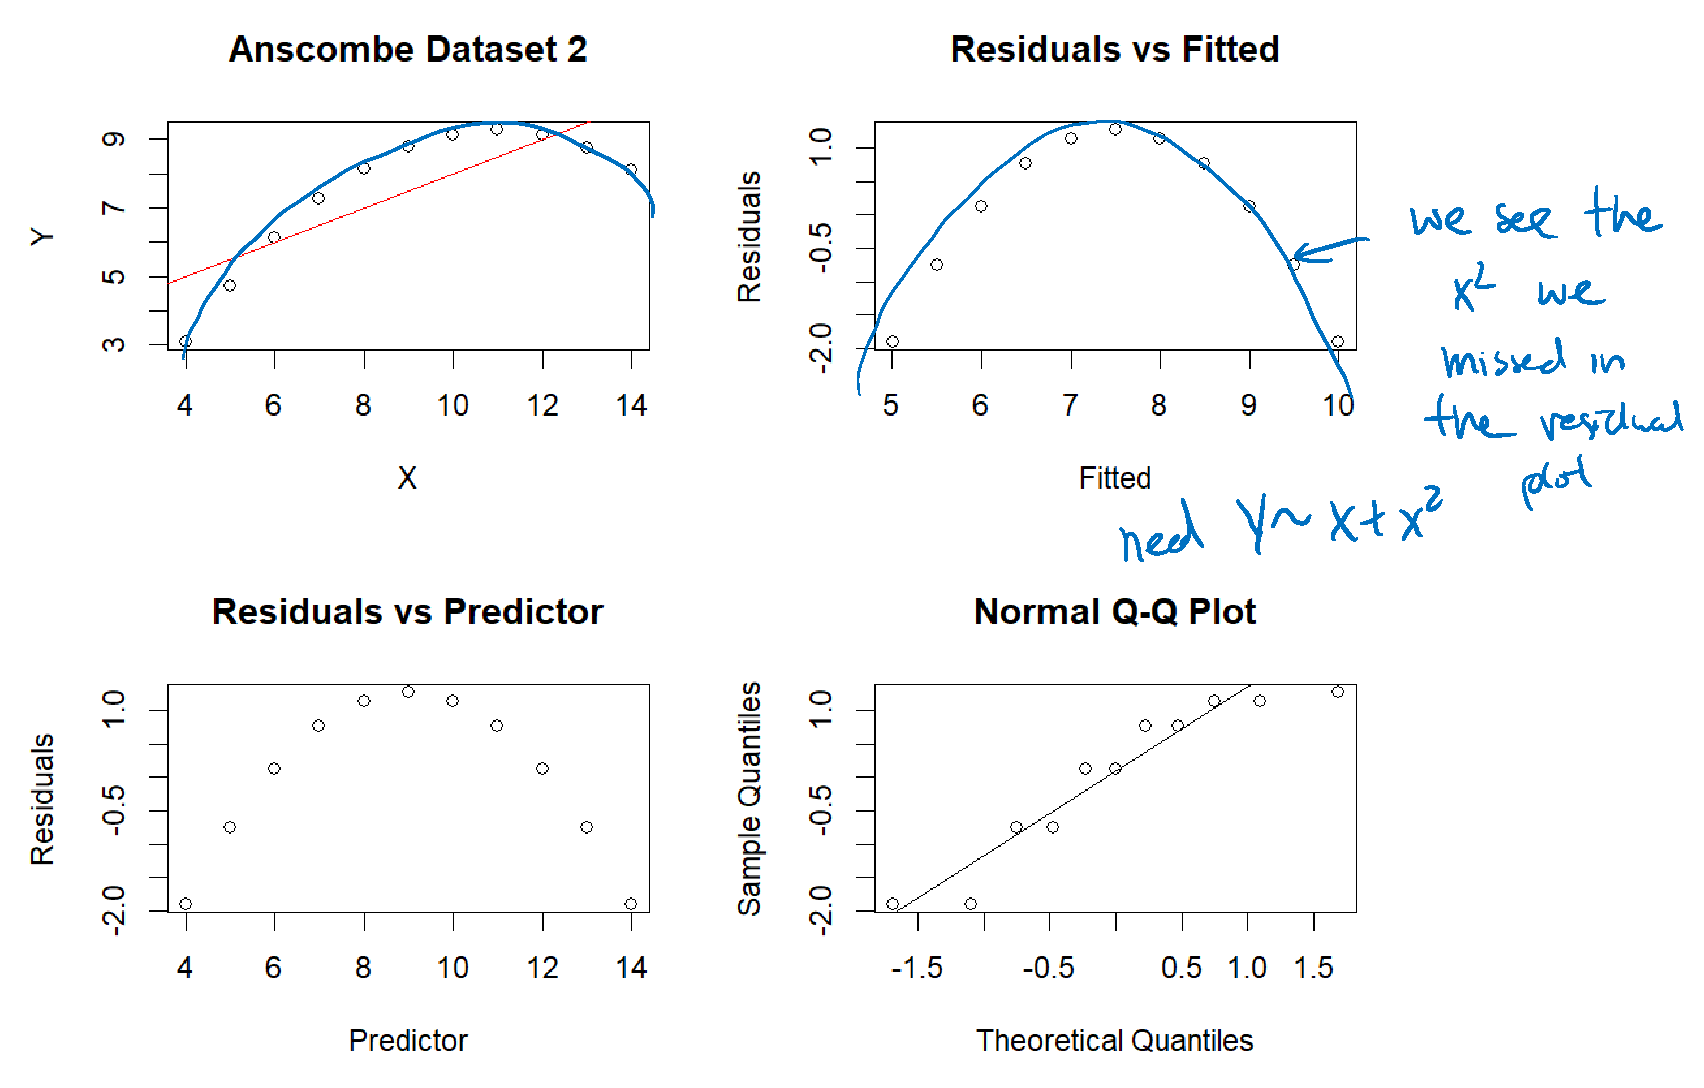
\includegraphics[width=\linewidth]{figures/anscombe2_diag.png}
            \\ \textit{\small Set 2: arch in the residuals}
        \end{minipage}
        \\[6pt]
        \begin{minipage}{0.48\linewidth}\centering
            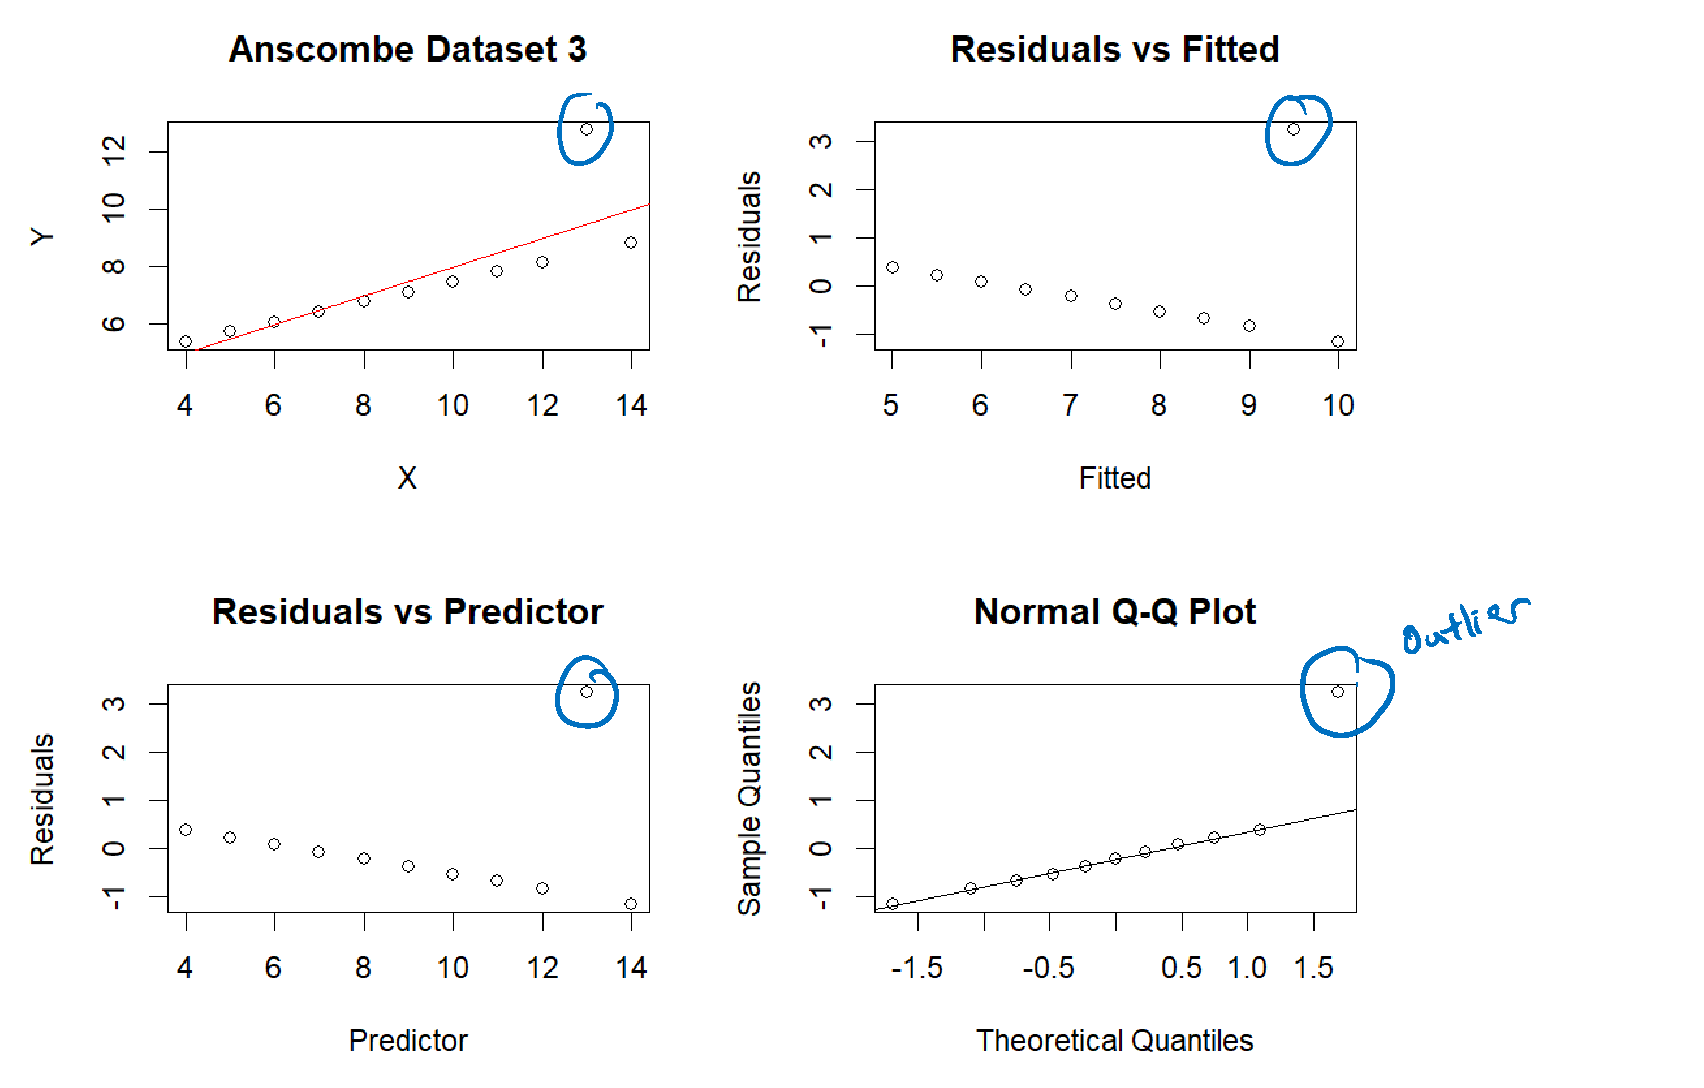
\includegraphics[width=\linewidth]{figures/anscombe3_diag.png}
            \\ \textit{\small Set 3: one outlier}
        \end{minipage}
        \hfill
        \begin{minipage}{0.48\linewidth}\centering
            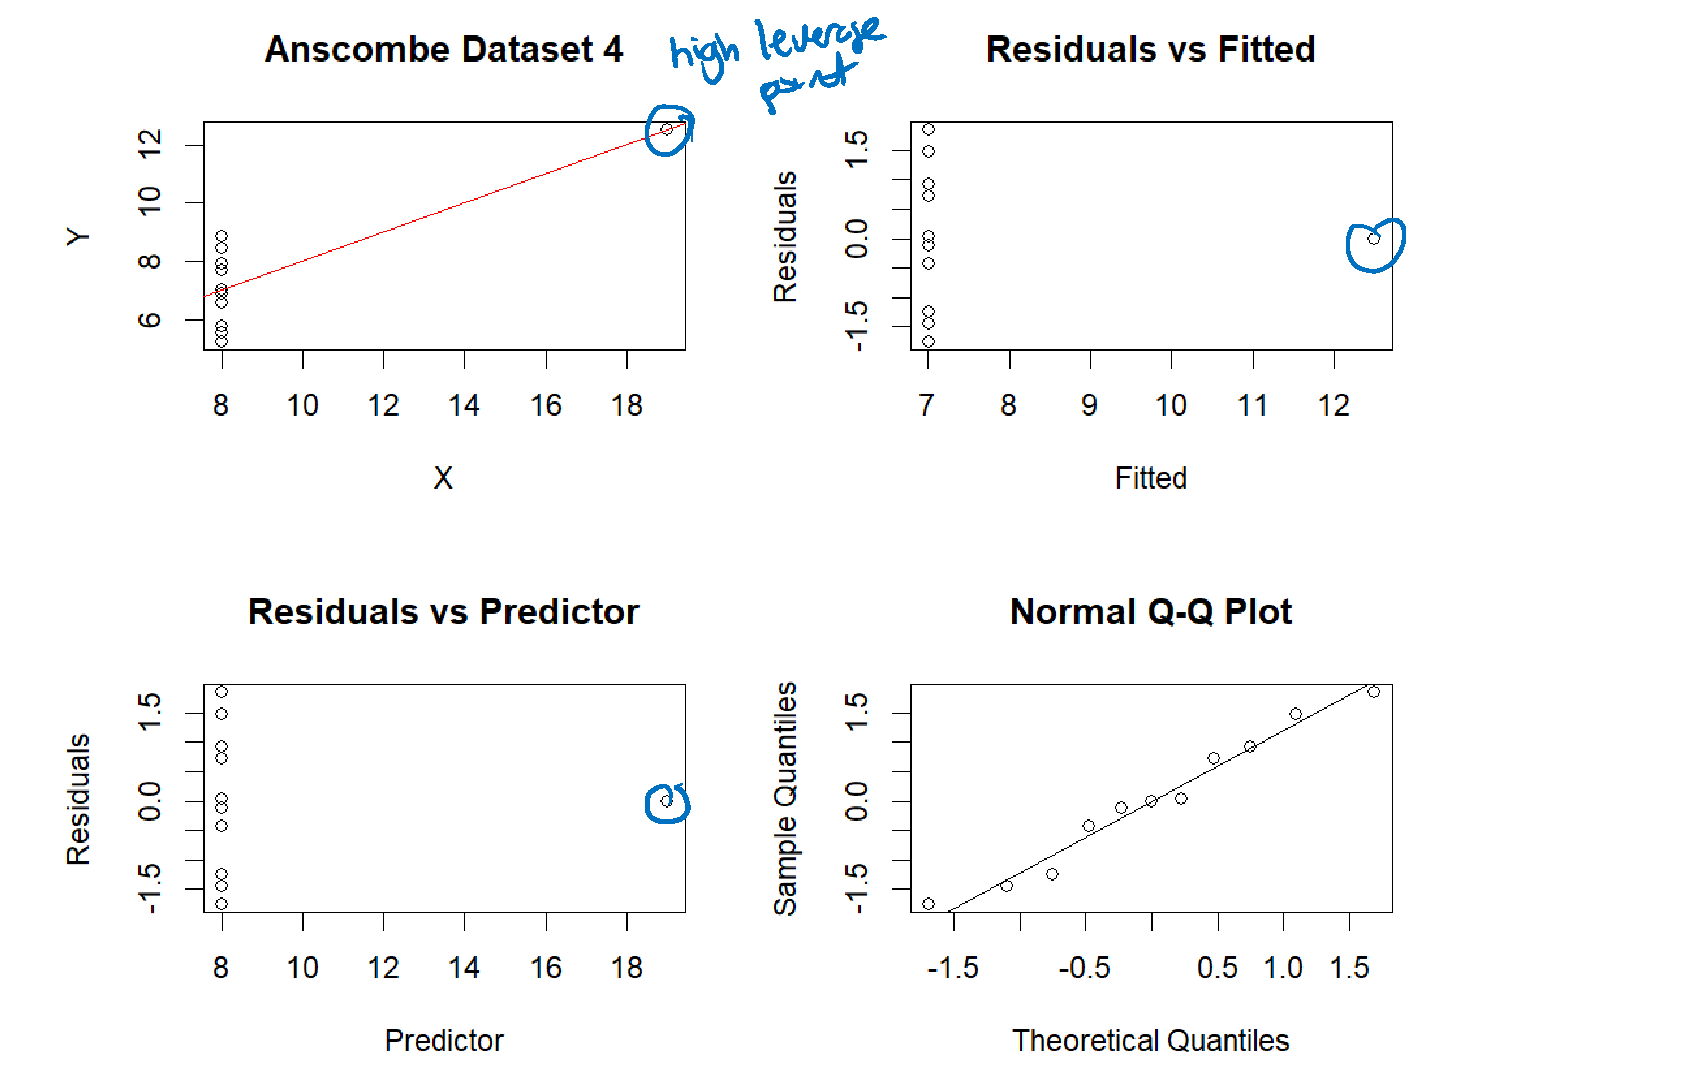
\includegraphics[width=\linewidth]{figures/anscombe4_diag.png}
            \\ \textit{\small Set 4: one high-leverage point}
        \end{minipage}
    \end{center}
    \aside{Set 2: we see the $x^2$ we missed in the residual plot --- need
    $Y\sim X+X^2$. Set 3: outlier stands out in every plot. Set 4: the
    high-leverage point at $x=19$ has residual $\approx0$ (since $h_{ii}\approx1$).}
\end{example}

\begin{remark}[Discrete Predictors]
    Random vertical ``bands'' of residuals indicate \textbf{no} violation
    when predictors are discrete (e.g.\ Michelin NY data,
    \texttt{lm(Price \textasciitilde\ Food + Decor + Service + InMichelin)}).
\end{remark}

\begin{center}
    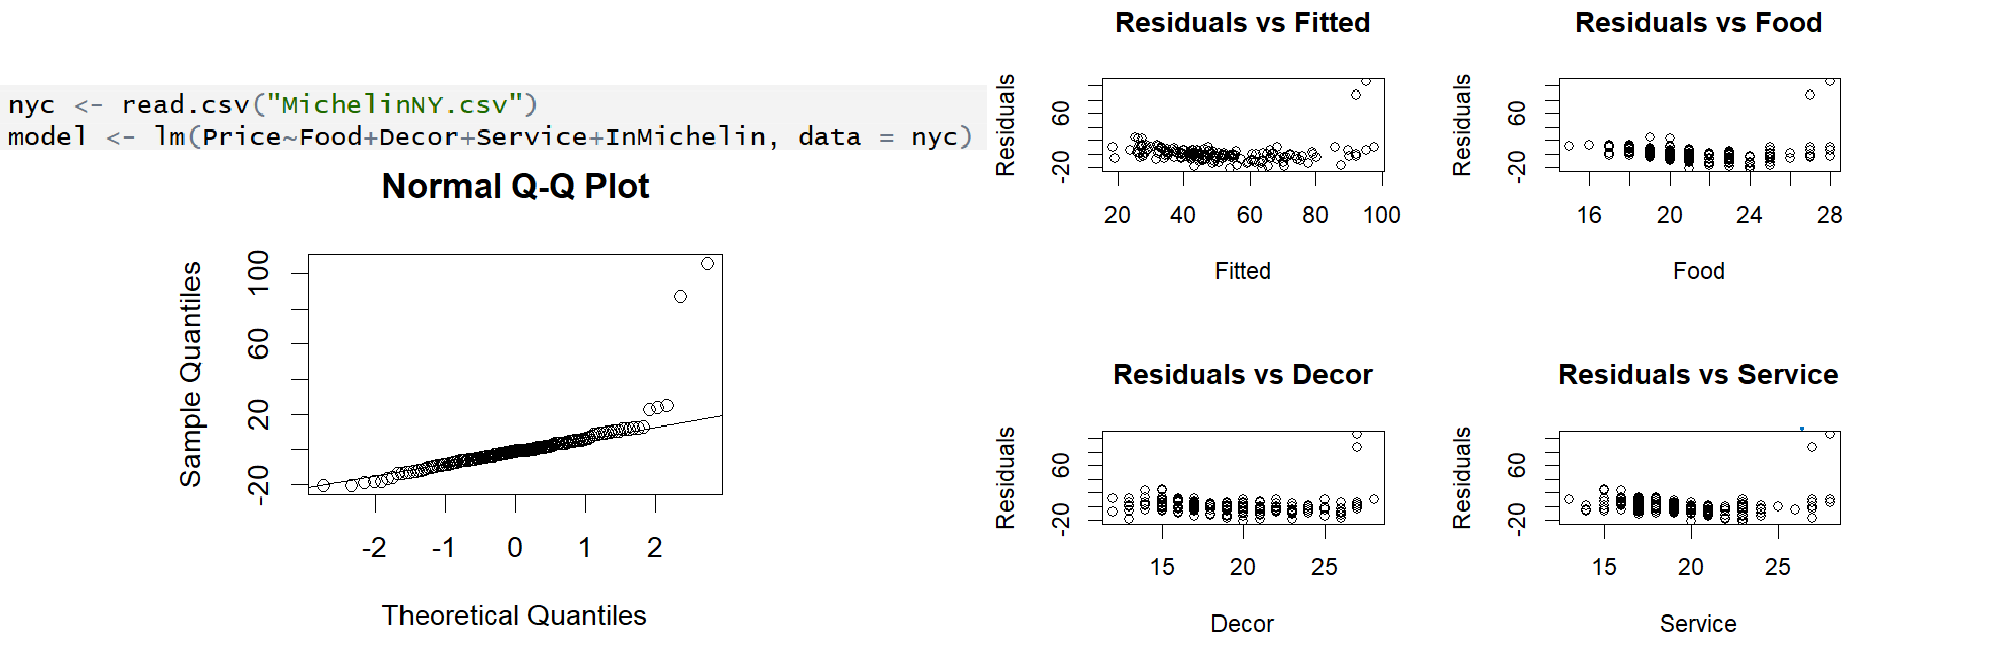
\includegraphics[width=0.8\linewidth]{figures/michelin_resid.png}
\end{center}

\heading{Explore and Understand the Data}
\begin{itemize}
    \item Do exploratory data analysis \emph{before} fitting a model --- plot plot plot!
    \begin{itemize}
        \item Is most of your data concentrated in a small area? Are the response or predictors skewed?
        \aside{Doesn't mean something is wrong, but look closer.}
    \end{itemize}
    \item Existing literature informs knowledge of the true relationship: what are the variables
    measuring? Are transformations typically done? What predictors mattered in prior studies?
    How should predictors be included?
\end{itemize}

\begin{example}[Think About the Data Collection Process]
    Which assumptions may be violated?
    \begin{itemize}
        \item ``Data was collected by voluntary response survey\dots''
        \\\db{Linearity: there could be response bias that isn't accounted for in the model.}
        \item ``Each variable was measured every day for a month\dots''
        \\\db{Uncorrelated errors (consecutive days are related).}
        \item ``Neighbourhoods were randomly sampled and all subjects from selected neighbourhoods were included\dots''
        \\\db{Uncorrelated errors (people in the same neighbourhood are related).}
    \end{itemize}
    Some violation is unavoidable (all models are wrong!) --- consider the
    context of the question and the cost of any errors.
\end{example}

\subsection{Additional Conditions for Multiple Regression Models}\label{sec:mlrconditions}

\aside{The instructor crossed out ``Linear'' in ``Multiple Linear Models'':
these conditions apply to multiple regression models in general.}

\begin{example}[What's Wrong Here?]
    The model $Y=\beta_0+\beta_1X_1+\beta_2X_2$ was fit, giving these residual plots:
    \begin{center}
        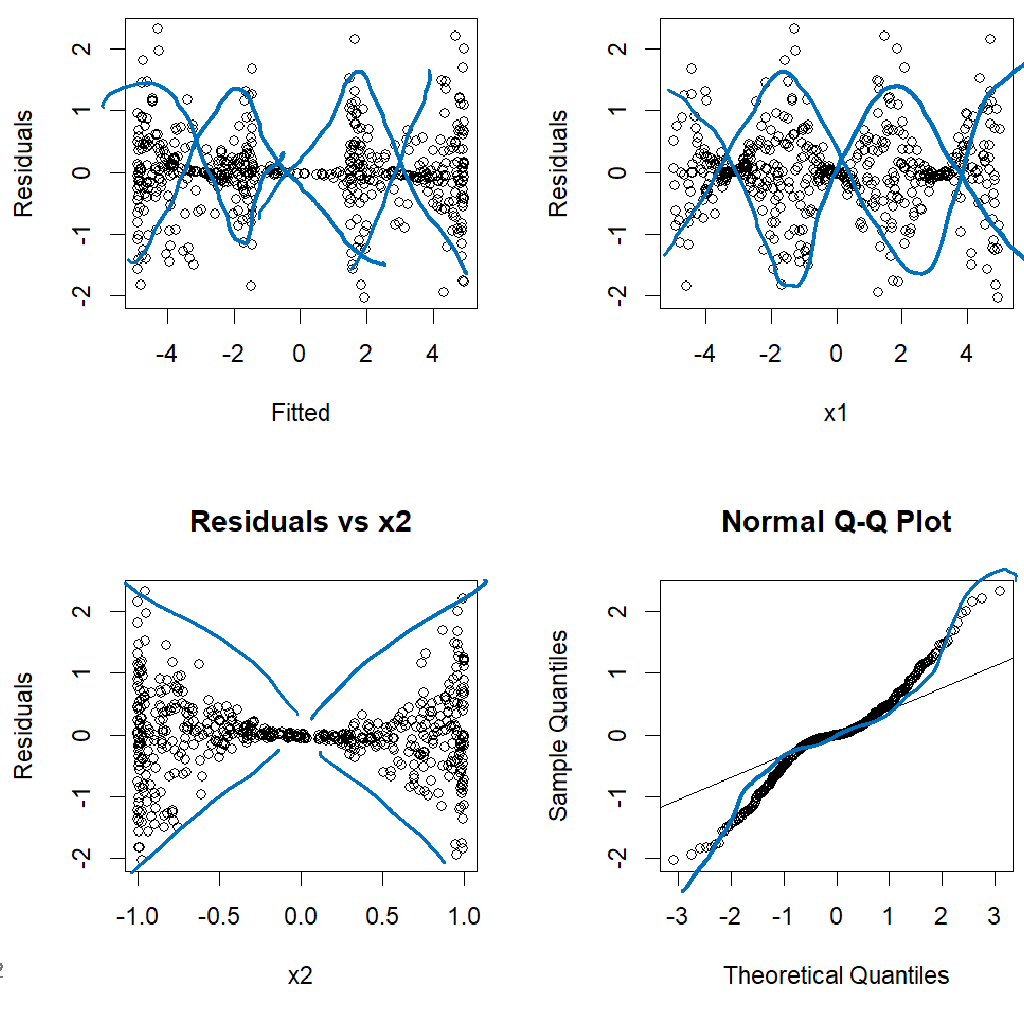
\includegraphics[width=0.55\linewidth]{figures/whats_wrong_resid.png}
    \end{center}
    The plots seem to suggest many violations (curved patterns, funnels,
    non-normal QQ). But the data were generated as
\begin{verbatim}
x1 = runif(n, -5, 5)
x2 = sin(x1)
Y  = x1 + 3*x2 + rnorm(n, 0, x2^2)
\end{verbatim}
    \db{The mean is correctly specified and the errors are normal and independent, so
    \dbb{non-constant variance} (sd $=x_2^2$) is the \emph{only} violated assumption.}
\end{example}

\begin{example}[Why Do We See More Issues Than the Funnel?]
    \begin{center}
        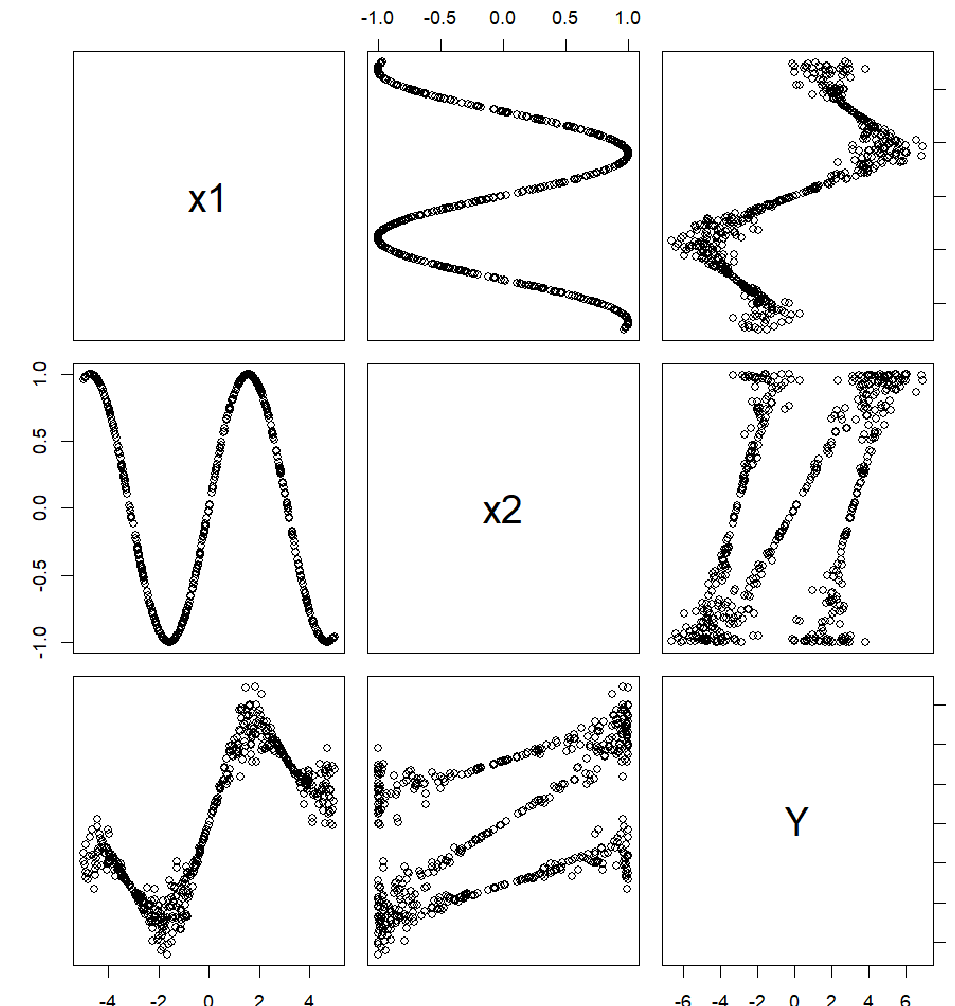
\includegraphics[width=0.45\linewidth]{figures/whats_wrong_pairs.png}
    \end{center}
    \db{The pairs plot shows $x_2=\sin(x_1)$: the predictors have a strongly
    \emph{non-linear} relationship. That makes the residual plots show patterns
    that are artifacts of the predictor relationship, not actual extra violations.}
\end{example}

\begin{definition}[Conditions for Interpreting Residual Plots in MLR]
    Coefficients are interpreted holding all other predictors fixed
    (conditioning on them). Before looking at residual plots, check
    (Li \& Duan, 1989; Sheather pg 155):
    \begin{enumerate}
        \item \rb{Conditional mean response condition}: the relationship
        between the response (or transformed response) and the predictors is linear,
        \[E(\mathbf{Y}\mid\mathbf{X}=\mathbf{x})=g(\beta_0+\beta_1x_1+\cdots+\beta_px_p)\]
        \item \rb{Conditional mean predictor condition}: each pair of
        predictors is linearly related,
        \[E(X_i\mid X_j)=\alpha_0+\alpha_1X_j\]
    \end{enumerate}
    \aside{These are for interpreting residual plots.}
\end{definition}

\begin{remark}[Why These Conditions?]
    \begin{itemize}
        \item More predictors $=$ more complexity. Residual plots may show
        patterns that are artifacts of relationships between predictors, not
        actual violations, and the pattern seen may not be what is actually
        missing or wrong.
        \item Recall: \hlt{violation of one assumption may affect the diagnostic plot for a separate assumption.}
        \item Complex relationships among predictors (or between predictors
        and response) make residual plots unreliable. Without checking both
        conditions, we \textbf{cannot} use residual plots to identify
        \emph{specific} violations.
    \end{itemize}
\end{remark}

\heading{How to Check}
\begin{itemize}
    \item \b{Response vs.\ fitted values}: identifies a non-linear relationship. Look for deviations from the line $\hat Y=Y$.
    \item \b{Pairs plot} (scatterplot matrix): identifies pairwise relationships between predictors. Look for curves and non-linear patterns.
\end{itemize}
\aside{Cook \& Weisberg (1999): ``Using residuals to guide model development
will often result in misdirection, or at best more work than would otherwise
be necessary.''}

\begin{example}[Both Conditions Hold --- NYC Italian Restaurants]
    3 numeric predictors (Food, Decor, Service) plus East (indicator).
    \begin{center}
        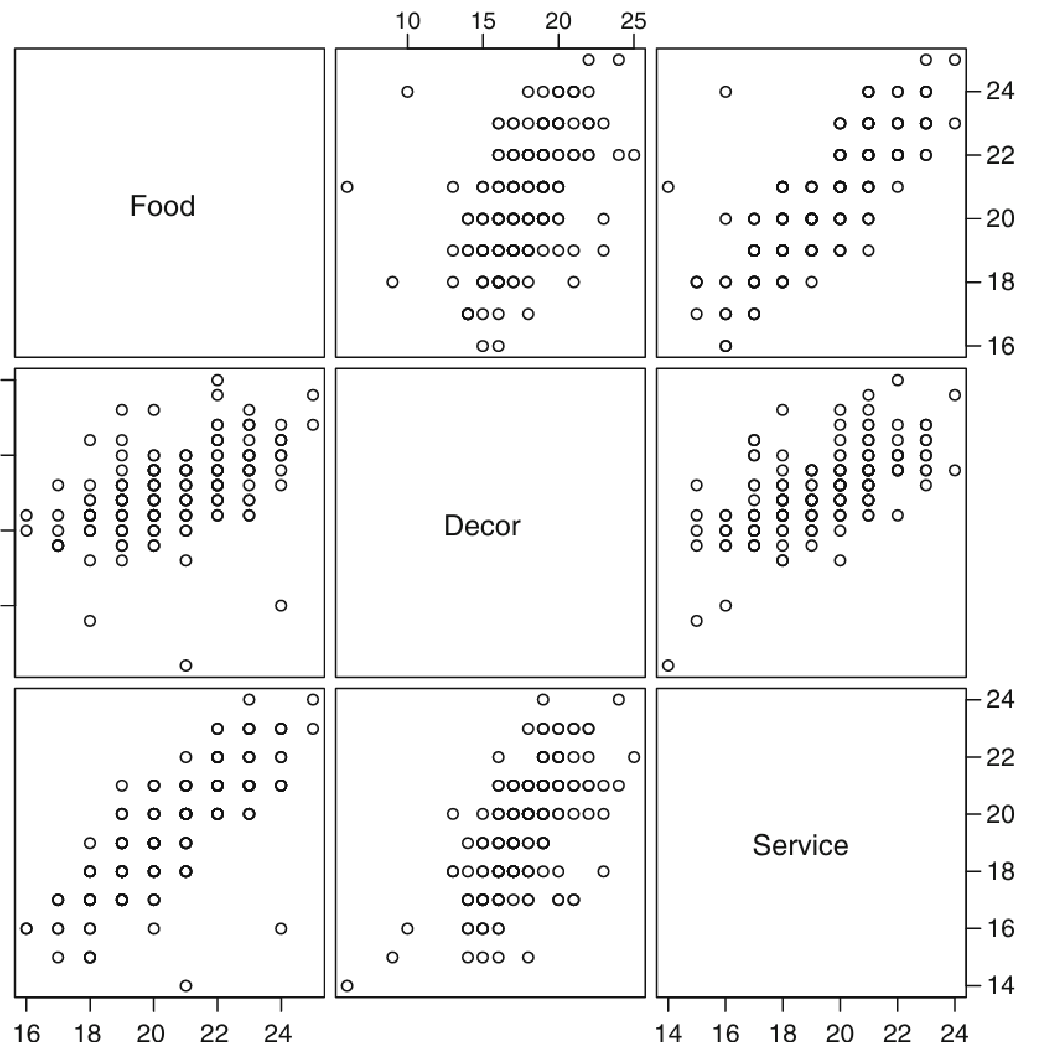
\includegraphics[width=0.42\linewidth]{figures/nyc_pairs.png}
    \end{center}
    The predictors are (approximately) linearly related $\Rightarrow$
    \textbf{conditional mean predictor condition holds}.
    \begin{center}
        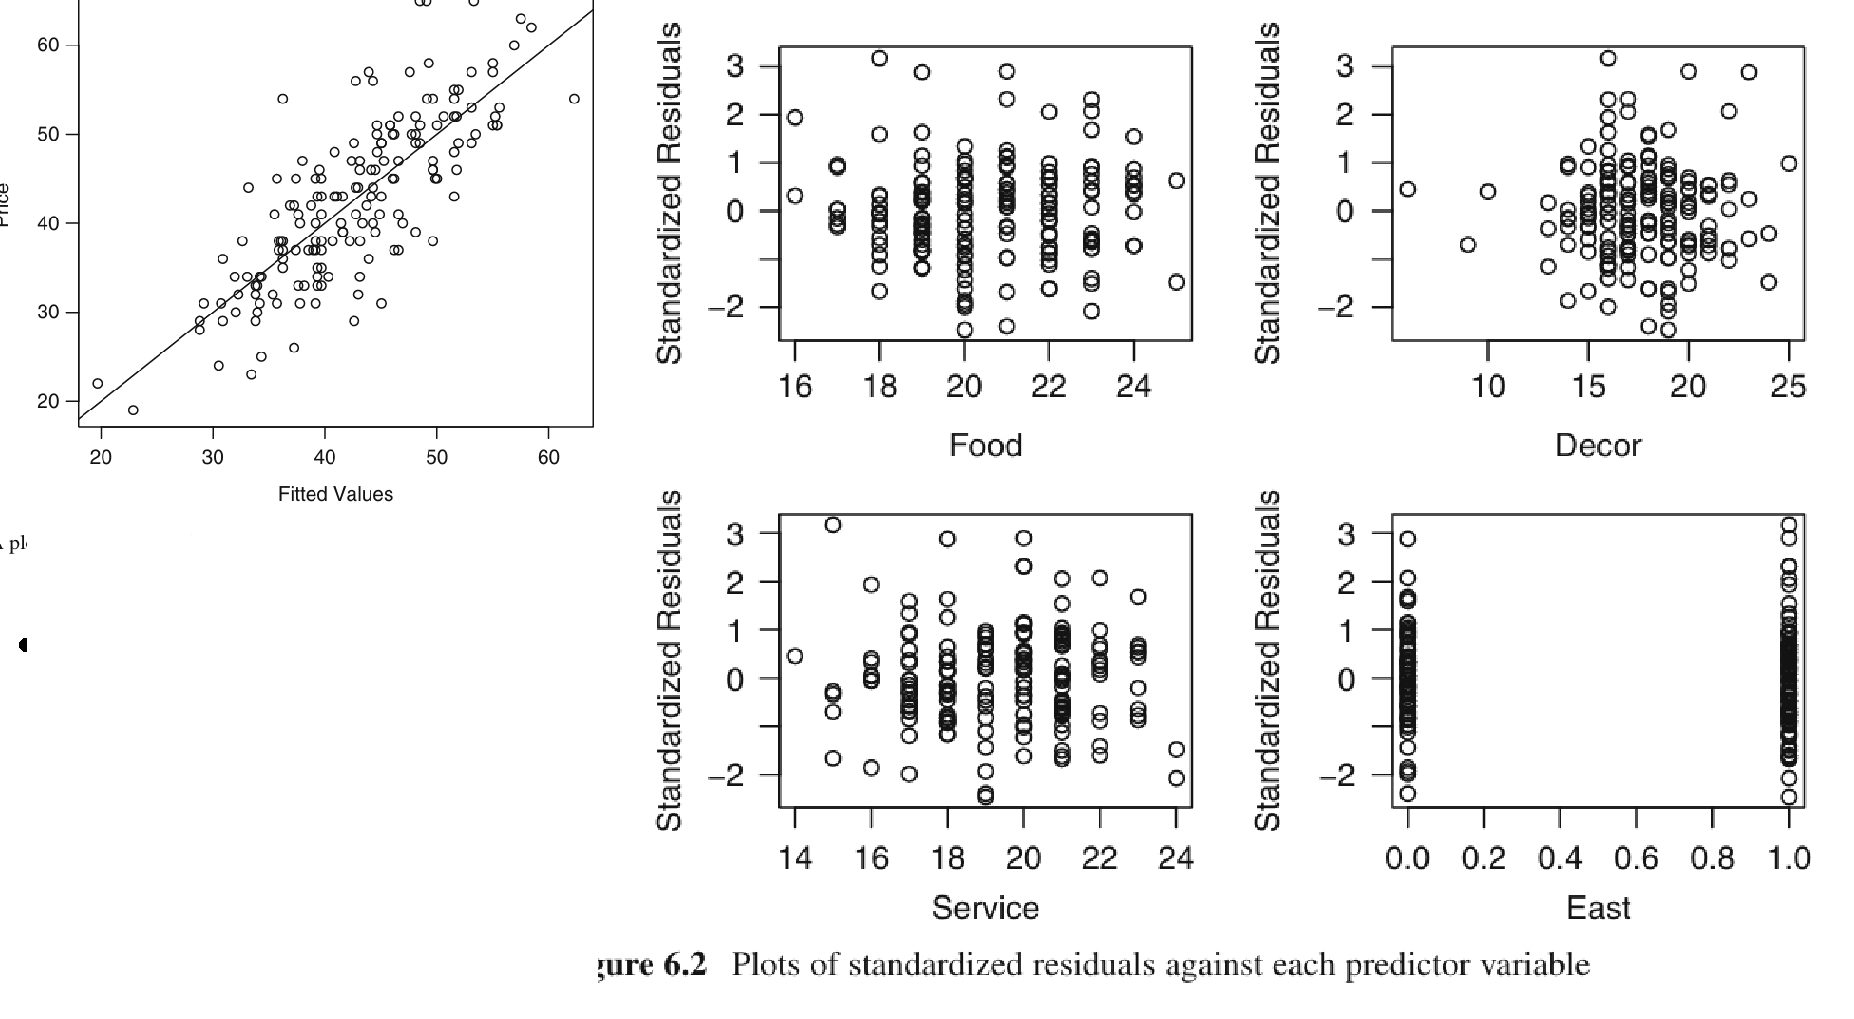
\includegraphics[width=0.85\linewidth]{figures/nyc_resid.png}
    \end{center}
    Price vs.\ fitted values follows the line $\Rightarrow$
    \textbf{conditional mean response condition holds} with $g(z)=z$, so
    the standardized residual plots can be trusted (and look fine).
\end{example}

\begin{example}[Conditional Mean Response Fails --- \texttt{alr4::caution}]
    (Sheather pg 159.) $x_1,x_2$ generated on the unit circle, errors
    i.i.d.\ $N(0,1)$, and
    \[E(Y\mid X)=\frac{|x_1|}{2+(1.5+x_2)^2}=\frac{g_1(x_1)}{g_2(x_2)},\]
    but the model fit is $Y=\beta_0+\beta_1x_1+\beta_2x_2+e$.
    \begin{center}
        \begin{minipage}{0.48\linewidth}\centering
            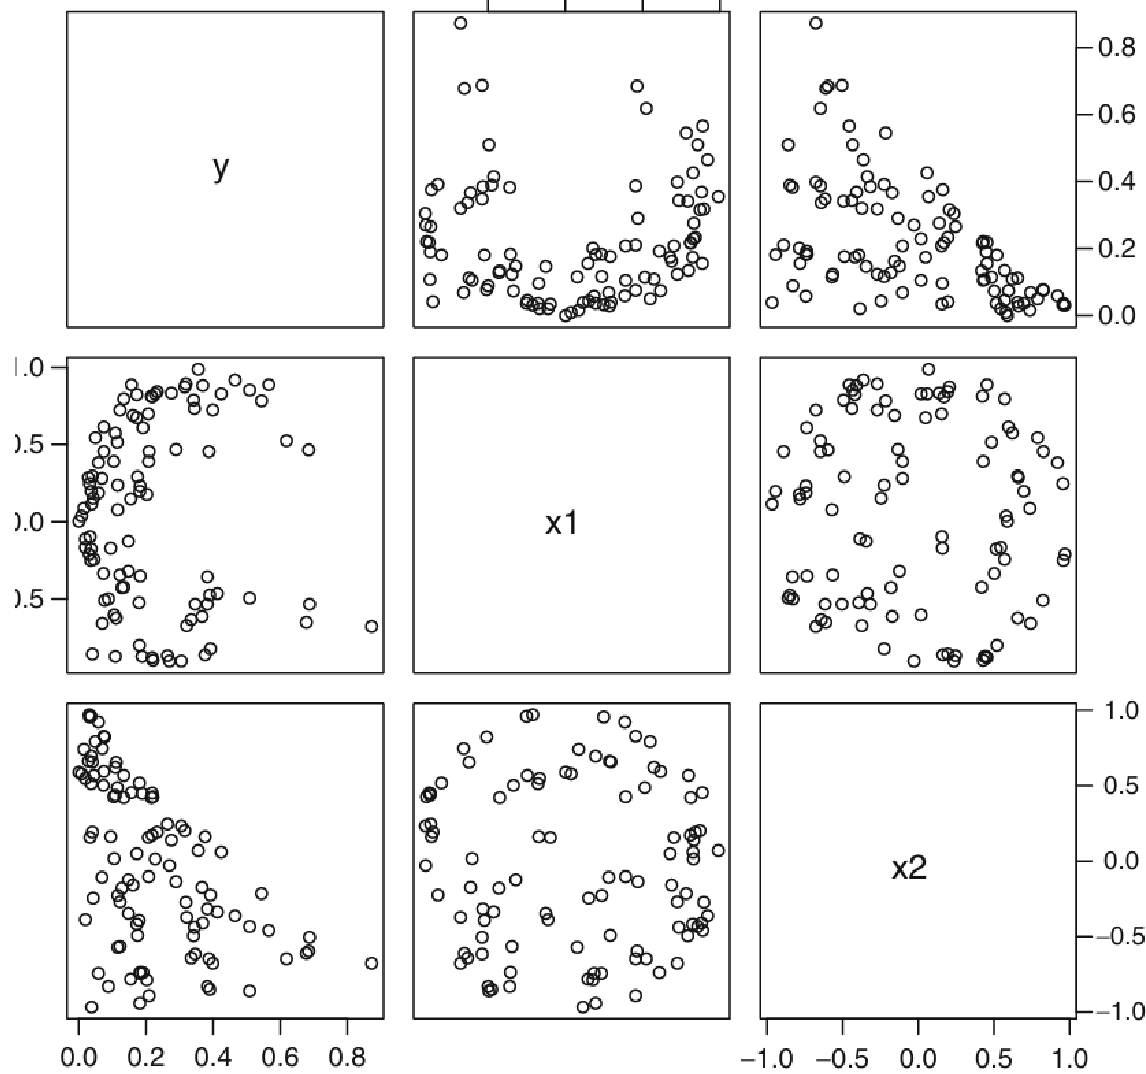
\includegraphics[width=\linewidth]{figures/caution_pairs.png}
        \end{minipage}
        \hfill
        \begin{minipage}{0.48\linewidth}\centering
            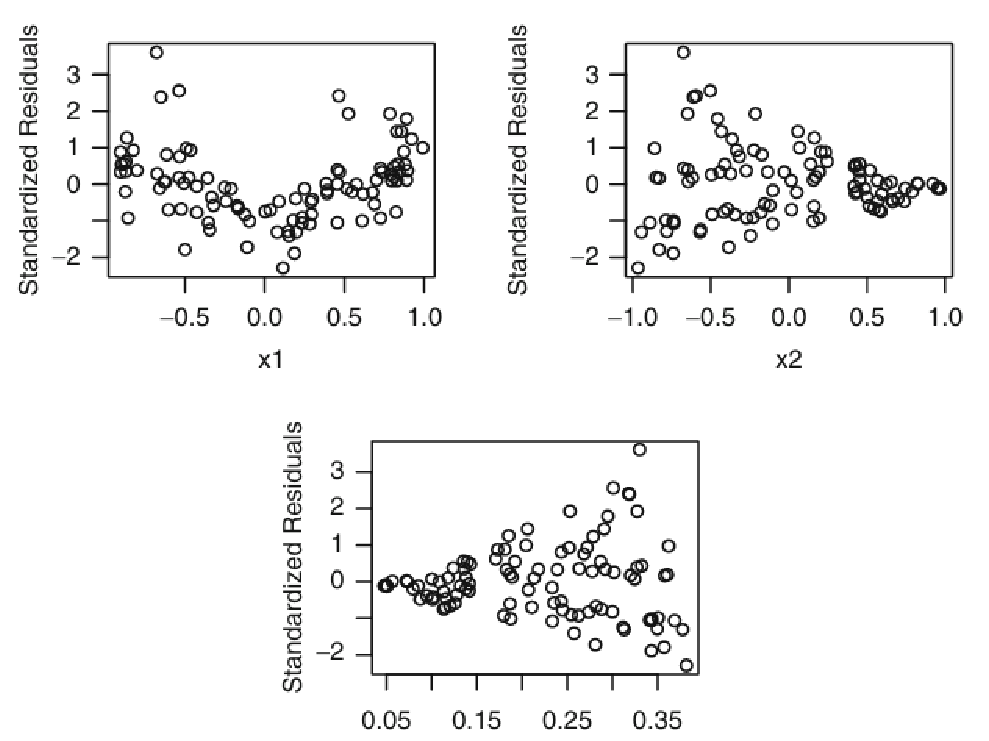
\includegraphics[width=\linewidth]{figures/caution_resid.png}
        \end{minipage}
    \end{center}
    \begin{itemize}
        \item $y$ has a complicated relationship with $x_1$ and $x_2$
        $\Rightarrow$ conditional mean response condition \textbf{violated}.
        \item Not enough visual evidence that $x_1$ vs.\ $x_2$ is non-linear
        $\Rightarrow$ conditional mean predictor condition holds.
        \item The residual plots look like a constant-variance problem, but
        we \emph{know} the errors are i.i.d.\ $N(0,1)$.
    \end{itemize}
    \db{\dbb{We can't say which part of the model is misspecified from the residual plots.}
    All we can say is that the model fit is invalid.}
\end{example}

\heading{Summary}
\begin{itemize}
    \item Choose which predictors to use (formal variable selection later)
    \item Fit the model
    \item Always plot (extensively!) to check whether the assumptions are valid
\end{itemize}

\begin{remark}[Module Takeaways]
    \begin{itemize}
        \item What are the assumptions of linear regression and what do they mean?
        \item What tools assess whether each assumption holds, and what do we look for?
        \item Why check the additional conditions in multiple regression models?
        \item What aspects of the data, data collection or population suggest an assumption may not hold?
    \end{itemize}
    \aside{Next week: correcting and mitigating violated assumptions.}
\end{remark}
